% Discription of what the Basler Camera is and how it is possible to use it in ROS

\chapter{Basler Camera\authorA}\label{ref:baslercamera}
One method that the model car of the Audi Autonomous Driving Cup (\gls{aadc}) 2018 uses to observe its surroundings is a camera. Without the car, another camera system has to be used for recording images. The camera on the \gls{aadc} 2018 car is a \textit{daA1280-54uc (S-Mount) - Basler dart} by the \textsc{Basler AG} \cite{daA12854uc}.

\section{Information}
The Camera is a 1.2 Megapixel CMOS camera that uses a USB 3.0 interface. It can do 54 \gls{fps} and features a global shutter which is very helpful \cite{baslerCamera}.
\begin{figure}[h]
	\centering
	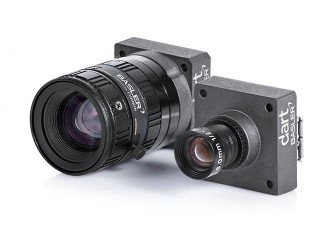
\includegraphics[height=0.3\textwidth]{./media/images/Basler-Camera.jpg}
  	\caption{Basler Camera
  	\\Src: \url{https://tinyurl.com/ss4mwzq}}
  	\label{orbslamkittidataset}
\end{figure}

\section{Prerequisites}
To use a Basler Camera in general it is required to have the so-called \textit{pylonSDK} installed which can be downloaded from the official \href{https://www.baslerweb.com/de/vertrieb-support/downloads/downloads-software/}{Basler homepage} \cite{pylonsdkdownloadpage}.

\section{Running pylon-ros-camera node}
The added node that fetches the video from the camera and then publishes it is called \textit{pylon-ros-camera} and is developed by the \textsc{Basler AG} since October 1st 2019 \cite{pylonroscamera}. Before a similar node was developed by the \textsc{Magazino GmbH}.\cite{pyloncamera}.

\subsection{Compiling node}

\begin{enumerate}
    \item \underline{Cloning Pylon Ros Camera} \newline
    First clone the \href{https://github.com/basler/pylon-ros-camera}{Github Repository} by the \cite{pylonroscamera} \textsc{Basler AG} into a workspace.
    
    \item \underline{Cloning DragAndBot\_common} \newline
    The DragAndBot\_common repository contains \textit{DragAndBot} messages and services that the pylon-\gls{ros}-camera node requires.
    So clone the \href{https://github.com/dragandbot/dragandbot_common}{\textit{DragandBot\_common} repository} \cite{dragandbotcommon} into the same workspace as the Pylon-Ros-Camera.
    
    \item \underline{Installing ROS dependencies} \newline
    To install the necessary dependencies for the \gls{ros} nodes using the command \cite{code:installdeppylonroscamera}.
    \begin{lstlisting}[language=bash, caption={Installing dependencies for Pylon-Ros-Camera}, label={code:installdeppylonroscamera}]
sudo sh -c 'echo "yaml https://raw.githubusercontent.com/basler/pylon-ros-camera/master/pylon_camera/rosdep/pylon_sdk.yaml" > /etc/ros/rosdep/sources.list.d/30-pylon_camera.list' && rosdep update && sudo rosdep install --from-paths . --ignore-src --rosdistro=$ROS_DISTRO -y
    \end{lstlisting}
    
    \item \underline{Compiling and Sourcing} \newline
    To compile the nodes run \textit{catkin build} or \textit{caktin\_make} in the root directory of the workspace.\newline
    To use the node when compiling has finished it is required to enter \textit{./devel/setup.bash} when being in the root directory.
\end{enumerate}

\subsection{Using Pylon-Ros-Camera Node}
Running the node is as simple as launching it by using \newline
\begin{lstlisting}[language=bash]
roslaunch pylon_camera pylon_camera_node.launch
\end{lstlisting}
This command published the video feed, which other nodes then can subscribe to.